\documentclass[10pt, compress]{beamer}

\usetheme[numbering=fraction, progressbar=frametitle]{metropolis}
\usepackage{booktabs}
\usepackage{array}
\usepackage{listings}
\usepackage{graphicx}
\usepackage[brazilian]{babel}
\usepackage[scale=2]{ccicons}
\usepackage{url}
\usepackage{relsize}
\usepackage{courier}

\usepackage{pgfplots}
\usepgfplotslibrary{dateplot}

\lstset{basicstyle=\footnotesize\ttfamily,breaklines=true}
\renewcommand*{\UrlFont}{\ttfamily\smaller\relax}

\graphicspath{{./img/}}

\title{INTRODUÇÃO À PROGRAMAÇÃO PARA GPUs USANDO CUDA}
\author{\footnotesize Pedro Bruel \\ {\scriptsize phrb@ime.usp.br}}
\institute{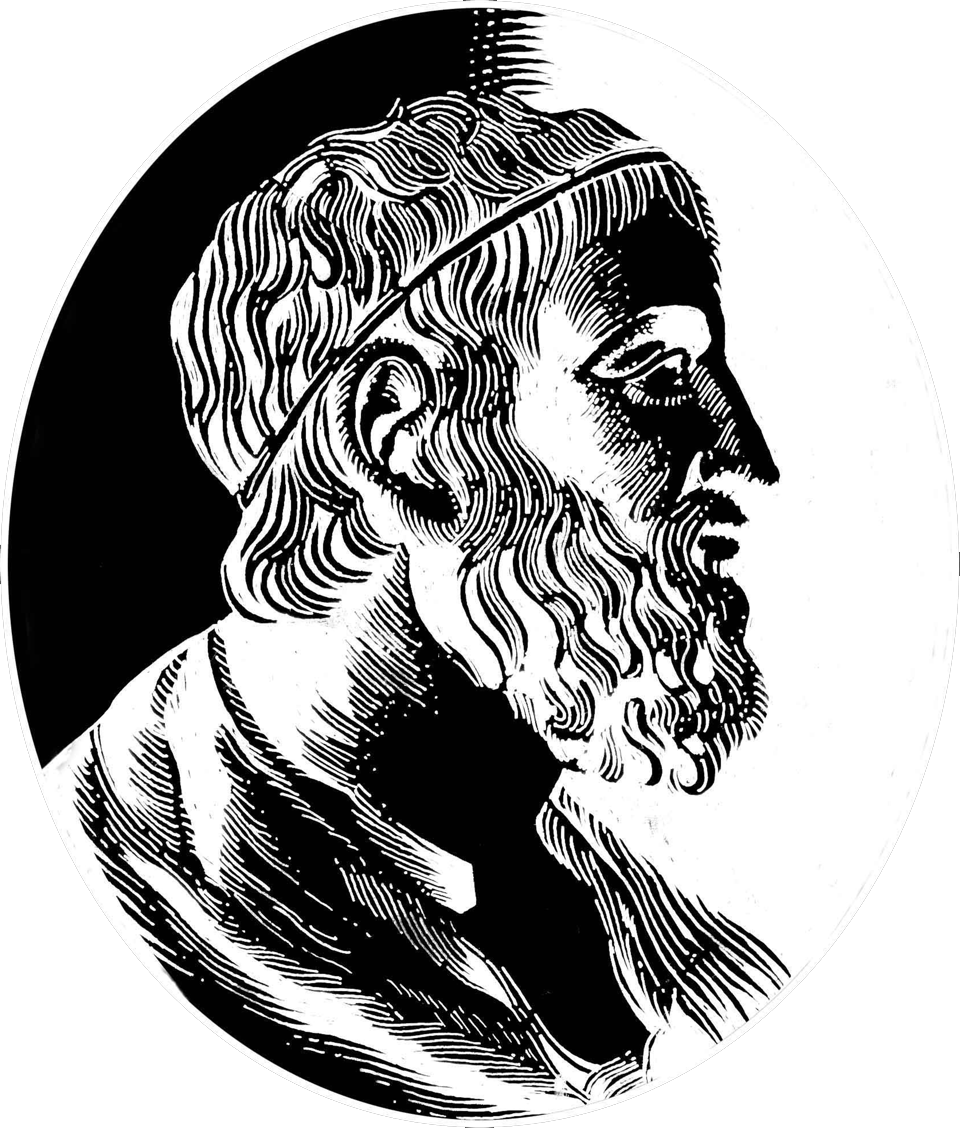
\includegraphics[height=2cm]{imelogo}\\[0.2cm] Instituto de Matemática e Estatística \\ Universidade de São Paulo}
\date{\scriptsize 29 de Setembro de 2015}

\begin{document}

\maketitle

\begin{frame}
    \frametitle{ROTEIRO}
    \setbeamertemplate{section in toc}[sections numbered]
    \begin{enumerate}
        \item Introdução
            \begin{itemize}
                \item \emph{Template} para programas CUDA
                \item \emph{Profilers} e \emph{Debuggers}
            \end{itemize}
            \pause
        \item Ferramentas
            \begin{itemize}
                \item \texttt{nvcc}
                \item \texttt{cuda-gdb}
                \item \texttt{cuda-memcheck}
            \end{itemize}
    \end{enumerate}
\end{frame}

\begin{frame}
    \frametitle{RECURSOS}

    Os \emph{pdf}s com as aulas e todo o código fonte usado nos exemplos estão
    no \alert{GitHub}:

    \begin{itemize}
        \item \url{github.com/phrb/aulas-gpu}
    \end{itemize}
    \pause

    Outros recursos:

    \begin{itemize}
        \item CUDA Toolkit Documentation: \url{docs.nvidia.com/cuda}
        \item GPU Teaching Kit: \url{syllabus.gputeachingkit.com}
        \item iPython: \url{ipython.org/notebook.html}
        \item CUDA Toolkit: \url{developer.nvidia.com/cuda-toolkit}
        \item Anaconda: \url{continuum.io/downloads}
    \end{itemize}
\end{frame}

\begin{frame}
    \frametitle{RECURSOS}
    
    Os próximos \emph{slides} foram adaptados do
    material disponível no \alert{GPU Teaching Kit}:
    \begin{itemize}
        \item \url{syllabus.gputeachingkit.com}
    \end{itemize}

\end{frame}

\plain{Obrigado!}

\maketitle

\end{document}
